\documentclass[12pt]{article}
\usepackage[utf8]{inputenc}
\usepackage[a4paper, margin=2cm]{geometry}
\usepackage[T1]{fontenc}
\usepackage{graphicx}
\usepackage{geometry}
\usepackage{amsmath}
\usepackage{amsfonts}
\usepackage{amssymb}
\usepackage{booktabs}
\usepackage{hyperref}
\usepackage{fancyhdr}
\usepackage{float}
\usepackage{ulem}
\usepackage{xeCJK}
\usepackage{listings}
\usepackage{xcolor}
\usepackage{indentfirst}
\setmainfont{Times New Roman}
\setCJKmonofont[BoldFont=SimHei, AutoFakeBold=true]{SimSun}
\lstset{
    basicstyle=\ttfamily\small,
    commentstyle=\color{gray},
    keywordstyle=\color{blue},
    stringstyle=\color{red},
    numberstyle=\tiny\color{gray},
    breaklines=true,
    captionpos=b,
    keepspaces=true,
    numbers=left,
    numbersep=5pt,
    showspaces=false,
    showstringspaces=false,
    showtabs=false,
    tabsize=2,
    frame=single,
    language=[x86masm]Assembler
}

\begin{document}
\thispagestyle{empty}

\begin{center}
    \vspace*{2cm}
    
    \Huge \textbf{2023-2024学年春季学期} \\
    \vspace{2cm}
    
    \Huge \textbf{《汇编语言程序设计》} \\
    \vspace{4cm}
    
    \large 评分：\underline{\hspace{4cm}} \\
    \vspace{6cm}
    
    \begin{tabular}{rl}
        \Large 学\hspace{2em}院： & \Large \underline{\makebox[12em][l]{\quad 计算机科学与工程学院}} \\
        \Large 专\hspace{2em}业： & \Large \underline{\makebox[12em][l]{\quad 计算机科学与技术}} \\
        \Large 班\hspace{2em}级： & \Large \underline{\makebox[12em][l]{\quad 计算机2204班}} \\
        \Large 姓\hspace{2em}名： & \Large \underline{\makebox[12em][l]{\quad 李俊洁}} \\
        \Large 学\hspace{2em}号： & \Large \underline{\makebox[12em][l]{\quad 20225443}} \\
        \Large 任课教师：         & \Large \underline{\makebox[12em][l]{\quad 刘思宇、柳秀梅}} \\
    \end{tabular}
    \vfill
\end{center}
\newpage

\section{实验目的}
本实验的主要目的是通过设计和实现一个驻留程序，深入理解中断处理机制及其在现代操作系统中的应用。
具体学习目标如下：

\begin{itemize}
    \item 掌握如何使用中断程序设计方法，尤其是如何创建和管理软件中断。
    \item 学习如何编写一个驻留程序，使其能够在不中断前台程序运行的情况下，持续执行特定功能。
    \item 实现一个实时时钟显示，能够在屏幕的右下角不断更新显示当前的时间（格式为HH:MM:SS），理解和应用中断驱动的界面更新技术。
    \item 增强对系统时钟中断处理和屏幕管理的理解，包括如何在中断服务程序中安全地进行屏幕操作。
    \item 开发中断服务程序时，学习如何保护CPU寄存器，确保中断处理的正确性和前台程序的稳定运行。
    \item 通过实际编码练习，提高解决实时系统问题的能力，如时间显示和中断同步。
\end{itemize}

\section{实验要求}
为确保实验的成功完成，并能够有效评估实验目的的实现程度，需遵守以下详细要求：
\begin{itemize}
    \item 编写一个驻留程序，该程序利用中断服务例程（ISR）在屏幕的右下角持续显示当前时间（HH:MM:SS格式）。
    \item 程序必须能够在不干扰当前运行的前台应用程序的情况下工作，确保前台程序的正常运行不受影响。
    \item 利用系统时钟中断（通常为INT 1Ch）来触发时间的更新，必须正确地挂接和恢复中断向量。
    \item 需要在屏幕的特定位置（右下角）显示时间，涉及屏幕坐标和输出的计算与管理。
    \item 确保时间更新过程中，屏幕的刷新不会导致闪烁或其他视觉上的干扰。
    \item 程序代码需要有清晰的注释，解释中断处理的流程和时间显示的方法。
    \item 程序结束后，需要能够安全地卸载驻留程序，并恢复所有更改过的中断向量及系统状态。
    \item 提交完整的源代码，以及详细的编译和运行指南，确保可以在标准的DOS环境下重现实验结果。
    \item 实验报告中应包括程序的流程图，详细描述程序的工作流程和中断处理策略。
    \item 必须记录并分析实验中遇到的任何问题及其解决方法，以反映问题解决和调试的过程。
\end{itemize}

\section{实验内容}
使用中断程序设计的方法，
编写一个驻留程序，
该程序可以在屏幕窗口的右下角显示当前的时间，
格式为HH:MM:SS，
时间的显示不能影响前台程序的正常运行。

\section{源程序}
    \begin{lstlisting}[caption={汇编源代码}, label=lst:asm2]
;数据段data
dseg segment
    count   dw 1
    time db '00:00:00',0dh,0ah,'$'    ;时间显示信息：hour:minute:second
dseg ends

sseg    segment  stack
    stack   db  100h  dup  (?)
sseg    ends

cseg segment
    assume  cs:cseg, ds:dseg
main proc near
start:
    ; 初始化
    mov     ax, dseg
    mov     ds, ax
    mov     ax, sseg
    mov     ss, ax
    mov     sp, 100h

    ; 保存原中断向量
    ; 将中断号1Ch（时钟滴答中断）加载到AL寄存器。
    ; 在此上下文中，AL寄存器用于指定接下来的DOS中断调用将操作哪个中断号。
    mov     al, 1ch
    ; 将 DOS 功能号35h加载到 AH 寄存器。AH为35h时，表示调用的是“获取中断向量”的功能。
    ; 允许程序查询系统中任何中断的当前处理程序地址。
    mov     ah, 35h
    int     21h                   ;获取1ch中断向量到es：bx
    ; 寄存器的内容推入堆栈，推栈操作保存值。
    ; 不加就按不了字符了
    push    es
    push    bx
    push    ds
    
    ;设置新的中断向量
    ; 这条指令将新的中断处理程序 intprocess 的偏移地址存储到 DX 寄存器中。
    ; offset 关键字用于获取标签或函数的内存偏移地址。
    mov     dx, offset intprocess
    ; 这条指令将新的中断处理程序 intprocess 的段地址存储到 AX 寄存器中
    ; seg 关键字用于获取标签或函数的段地址。
    mov     ax, seg intprocess
    ; 这条指令设置数据段寄存器 DS 为新的中断处理程序的段地址
    ; 因为 DOS 中断 25h 使用 DS:DX 作为参数来设置中断向量。
    mov     ds, ax
    ; 加载 1Ch 中断号到 AL 寄存器，指定要设置的是哪一个中断向量。
    mov     al, 1ch
    ; 将 DOS 功能号 25h（设置中断向量）加载到 AH 寄存器。
    mov     ah, 25h
    int     21h                   ;设置中断向量ds：dx
    pop     ds
    in      al, 21h               ;读中断屏蔽寄存器
    ; 通过逻辑与操作清除屏蔽寄存器中的最低位，即允许中断 0 （通常是系统时钟中断）发生。
    ; 位掩码 11111110b 确保除了最低位外的所有位保持不变，从而只允许相关的中断。
    and     al, 11111110b         ;开定时器中断
    out     21h, al               ;写中断屏蔽寄存器
    sti                           ;开中断
;等待中断
do_while:
    mov     ah, 1
    int     21h
    cmp     al, 'q'                ;'q'退出
    jz      quit
    jmp     do_while
;恢复
quit:
    pop     dx
    pop     ds
    mov     al, 1ch ; 时钟滴答中断
    mov     ah, 25h ; 设置中断向量
    int     21h ; 中断向量恢复
    ;调色、位置（跳出时钟效果后的背景色以及字体颜色）
    mov     ah, 00h ; 设置视频模式
    mov     al, 03h ; 文本模式
    int     10h
    mov     ah, 6
    mov     al, 0                 ; 屏幕为空白
    mov     bh, 00000111b         ; 背景色恢复
    mov     ch, 0                 ; 左上角x坐标
    mov     cl, 0                 ; 左上角y坐标
    mov     dh, 99h               ; 右下角x坐标
    mov     dl, 99h               ; 右下角y坐标
    int     10h
    ; 结束程序
    mov     ah, 4ch
    int     21h
main endp

intprocess proc near
    ; 保护数据
    push    ds
    push    ax
    push    bx
    push    cx
    push    dx

    sti     ; 该指令设置处理器的中断标志，允许中断被处理
    dec     count ; 计数器减一
    jnz     exit
    call    displaytime ; 为0显示时间
    mov     count, 18 ; 计数器加
exit:    
    cli ; 关闭中断
    pop     dx
    pop     cx
    pop     bx
    pop     ax
    pop     ds
    iret ; 中断服务例程的标准结束指令
intprocess endp

displaytime proc near
    push    ax
    push    bx
    push    cx
    push    dx
    push    si
    ;获取系统时间：
    ; 入口：ah存2ch
    ; ch存hour
    ; cl存minute
    ; dh存second
    mov     ah, 2ch ; 设置AH寄存器为 2ch，用于获取系统时间。
    ; 调用中断 21h 执行获取时间的功能
    ; 返回的时间将被存放在 ch、cl 和 dh 寄存器中，分别表示小时、分钟和秒。
    int     21h
    ; 小时
    mov     bl, 10                ; 用作后面的除法运算基数
    lea     si, time              ; 读文件
    mov     al, ch                ; 处理小时
    xor     ah, ah                ; 清除高位
    div     bl                    ; 执行除法
    add     al, 30h               ; 转ASCII
    add     ah, 30h               ; 转ASCII
    mov     [si], ax              ; 储存
    ; 分
    add     si, 3                 ; 指针移动，处理分钟
    mov     al, cl                ; 处理分钟
    xor     ah, ah                ; 清除高位
    div     bl                    ; 执行除法
    add     al, 30h               ; 转ASCII
    add     ah, 30h               ; 转ASCII
    mov     [si], ax              ; 储存
    ; 秒
    add     si, 3                 ; 指针移动，处理秒钟
    mov     al, dh                ; 处理秒钟
    xor     ah, ah                ; 清除高位
    div     bl                    ; 执行除法
    add     al, 30h               ; 转ASCII
    add     ah, 30h               ; 转ASCII
    mov     [si], ax              ; 储存
    ; 显示
    mov     ah, 02h               ; 设置AH寄存器为 02h，用于显示字符串。
    mov     bh, 0h                ; 页号
    mov     dh, 17h               ; 行号
    mov     dl, 42h               ; 列号
    int     10h

    ; 放置一个窗口遮罩
    mov     ah, 6
    mov     al, 0                 ; 屏幕为空白
    mov     bh, 01110000b         ; 背景色0000黑色
    mov     ch, 0                 ; 左上角x坐标
    mov     cl, 0                 ; 左上角y坐标
    mov     dh, 99h               ; 右下角x坐标
    mov     dl, 99h               ; 右下角y坐标
    int     10h

    ;显示时间字符串
    mov     dx, offset time       ; 提取最终要显示的时间
    mov     ah, 09h               ; 中断21h，用于显示字符串直到遇到$
    int     21h
    
    pop     si
    pop     dx
    pop     cx
    pop     bx
    pop     ax
    ret
displaytime endp

cseg ends
    end     start
    \end{lstlisting}

\section{运行结果}
    \subsection{调试步骤}
    每次调试程序所输入的数据以及显示器上输出的结果:

    \begin{center}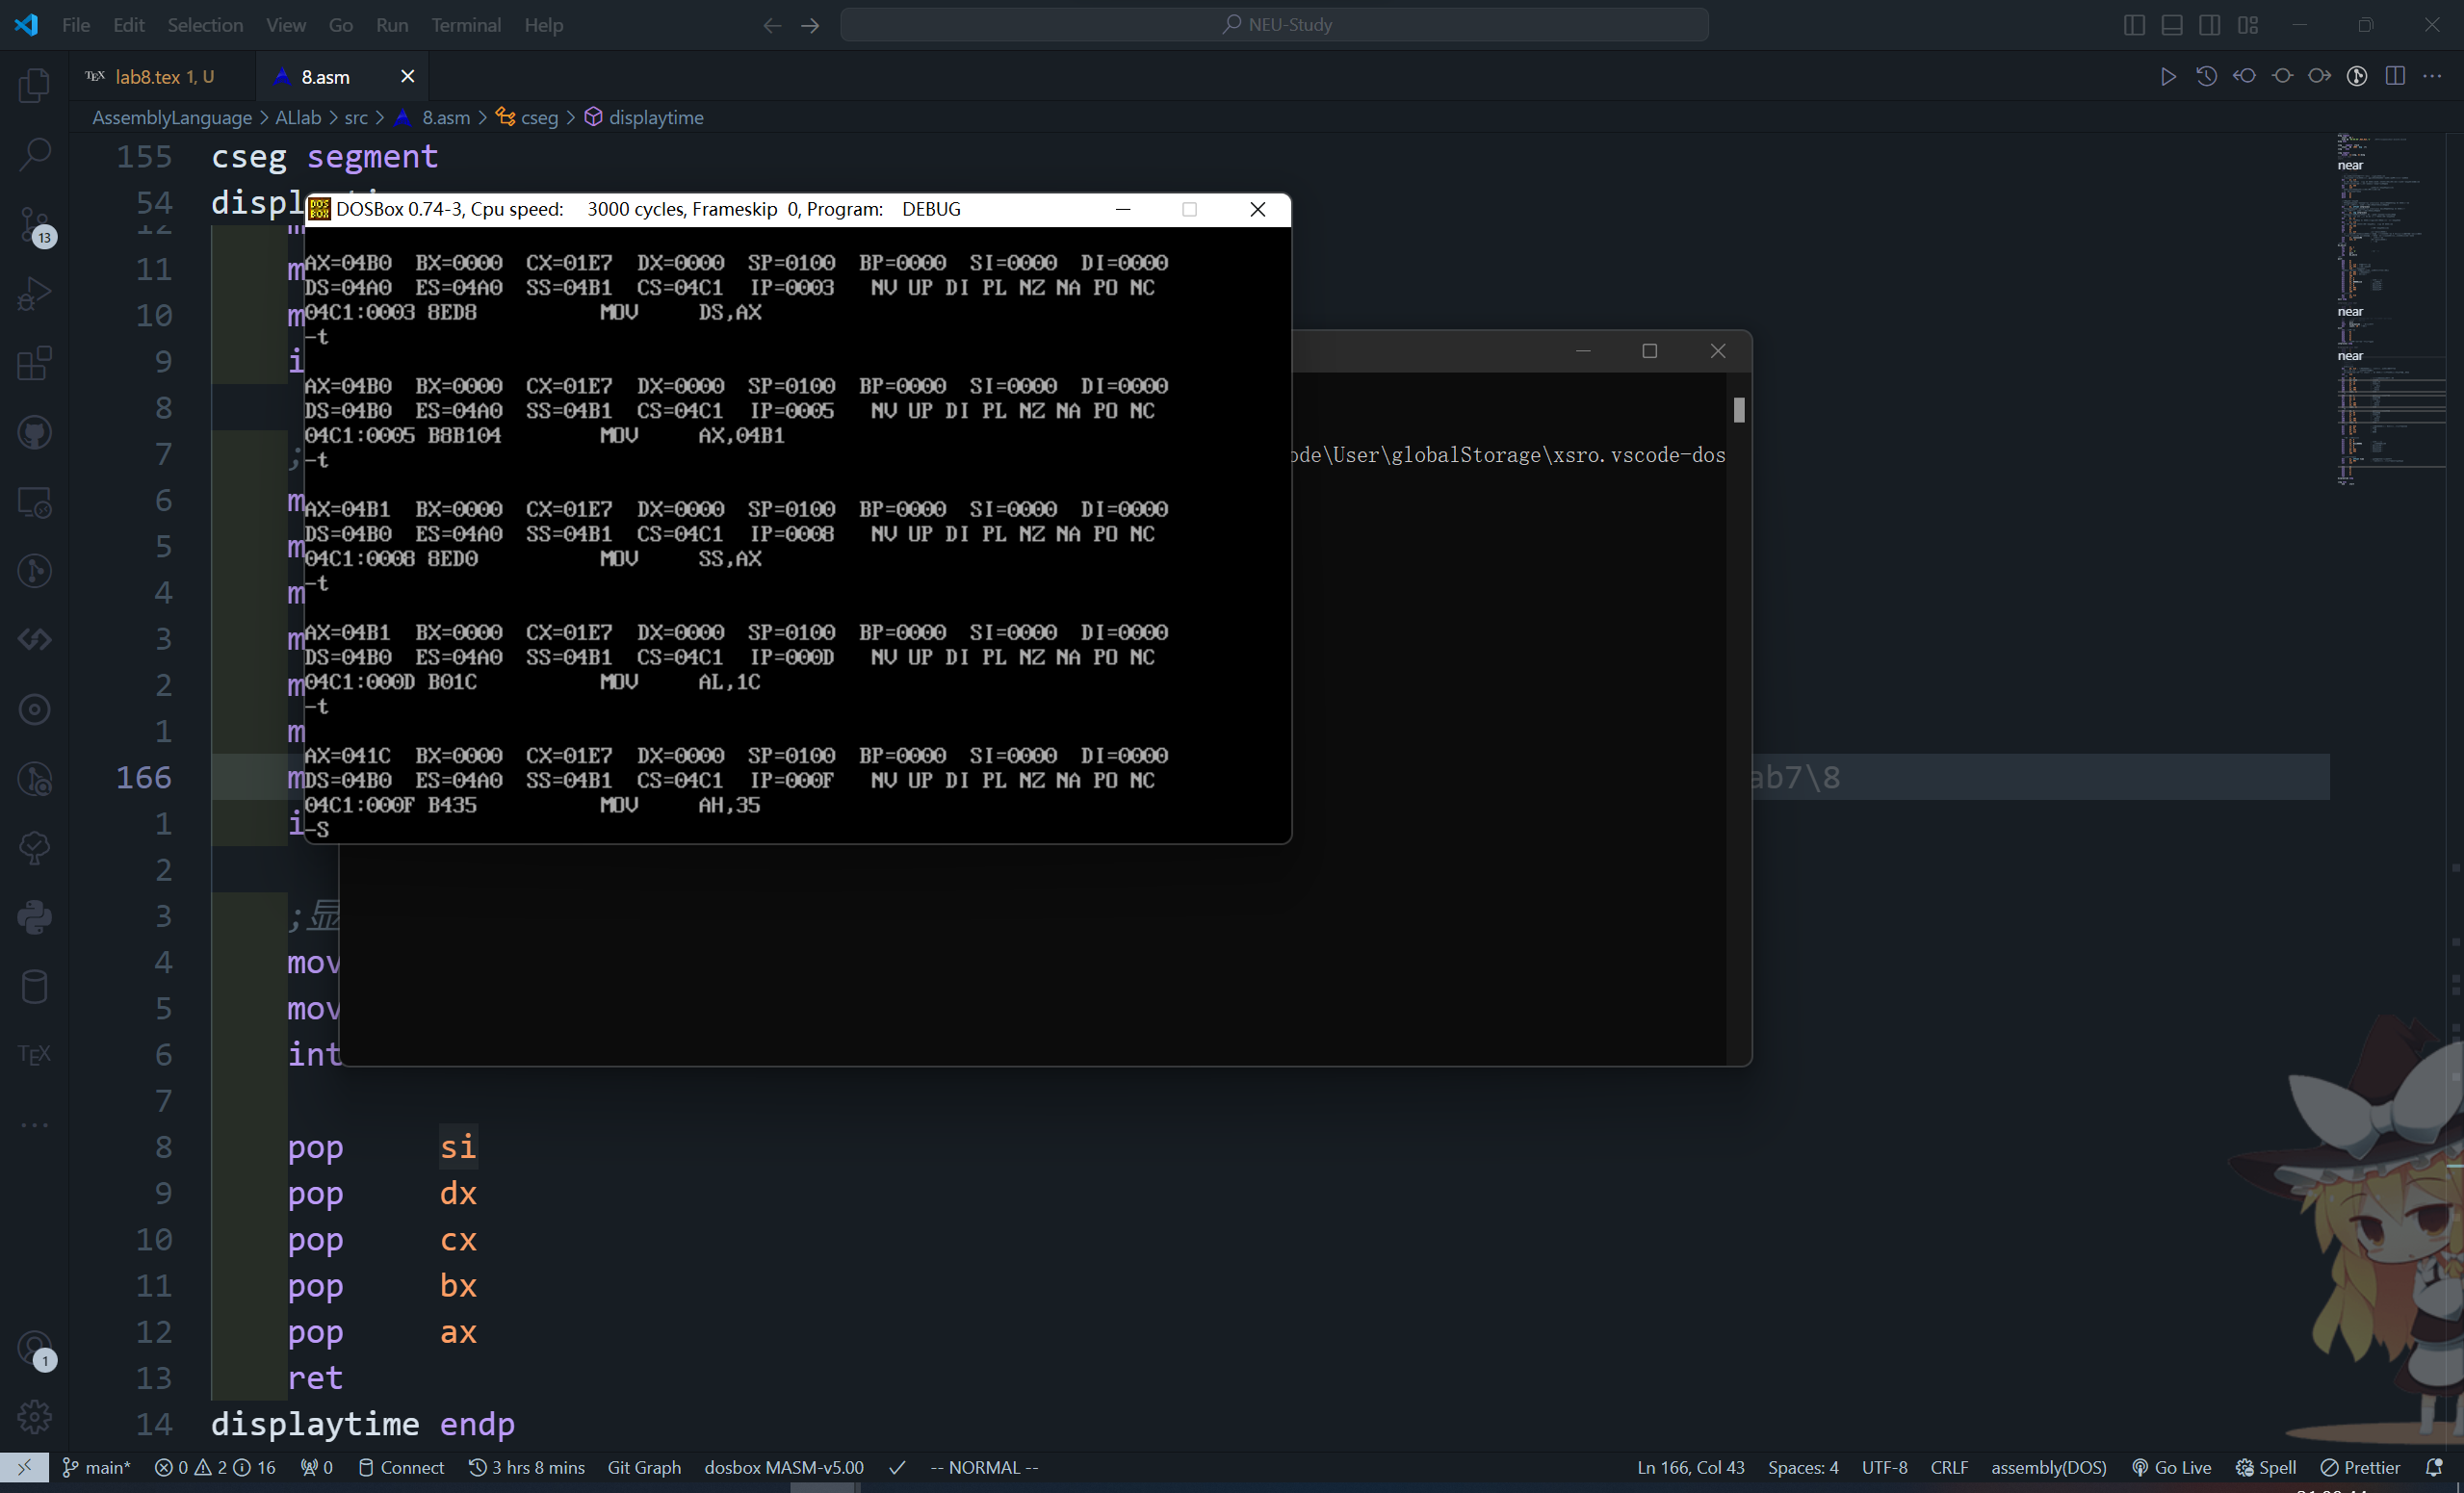
\includegraphics[width=1\textwidth]{image/AL_69.png}\end{center}
    \begin{center}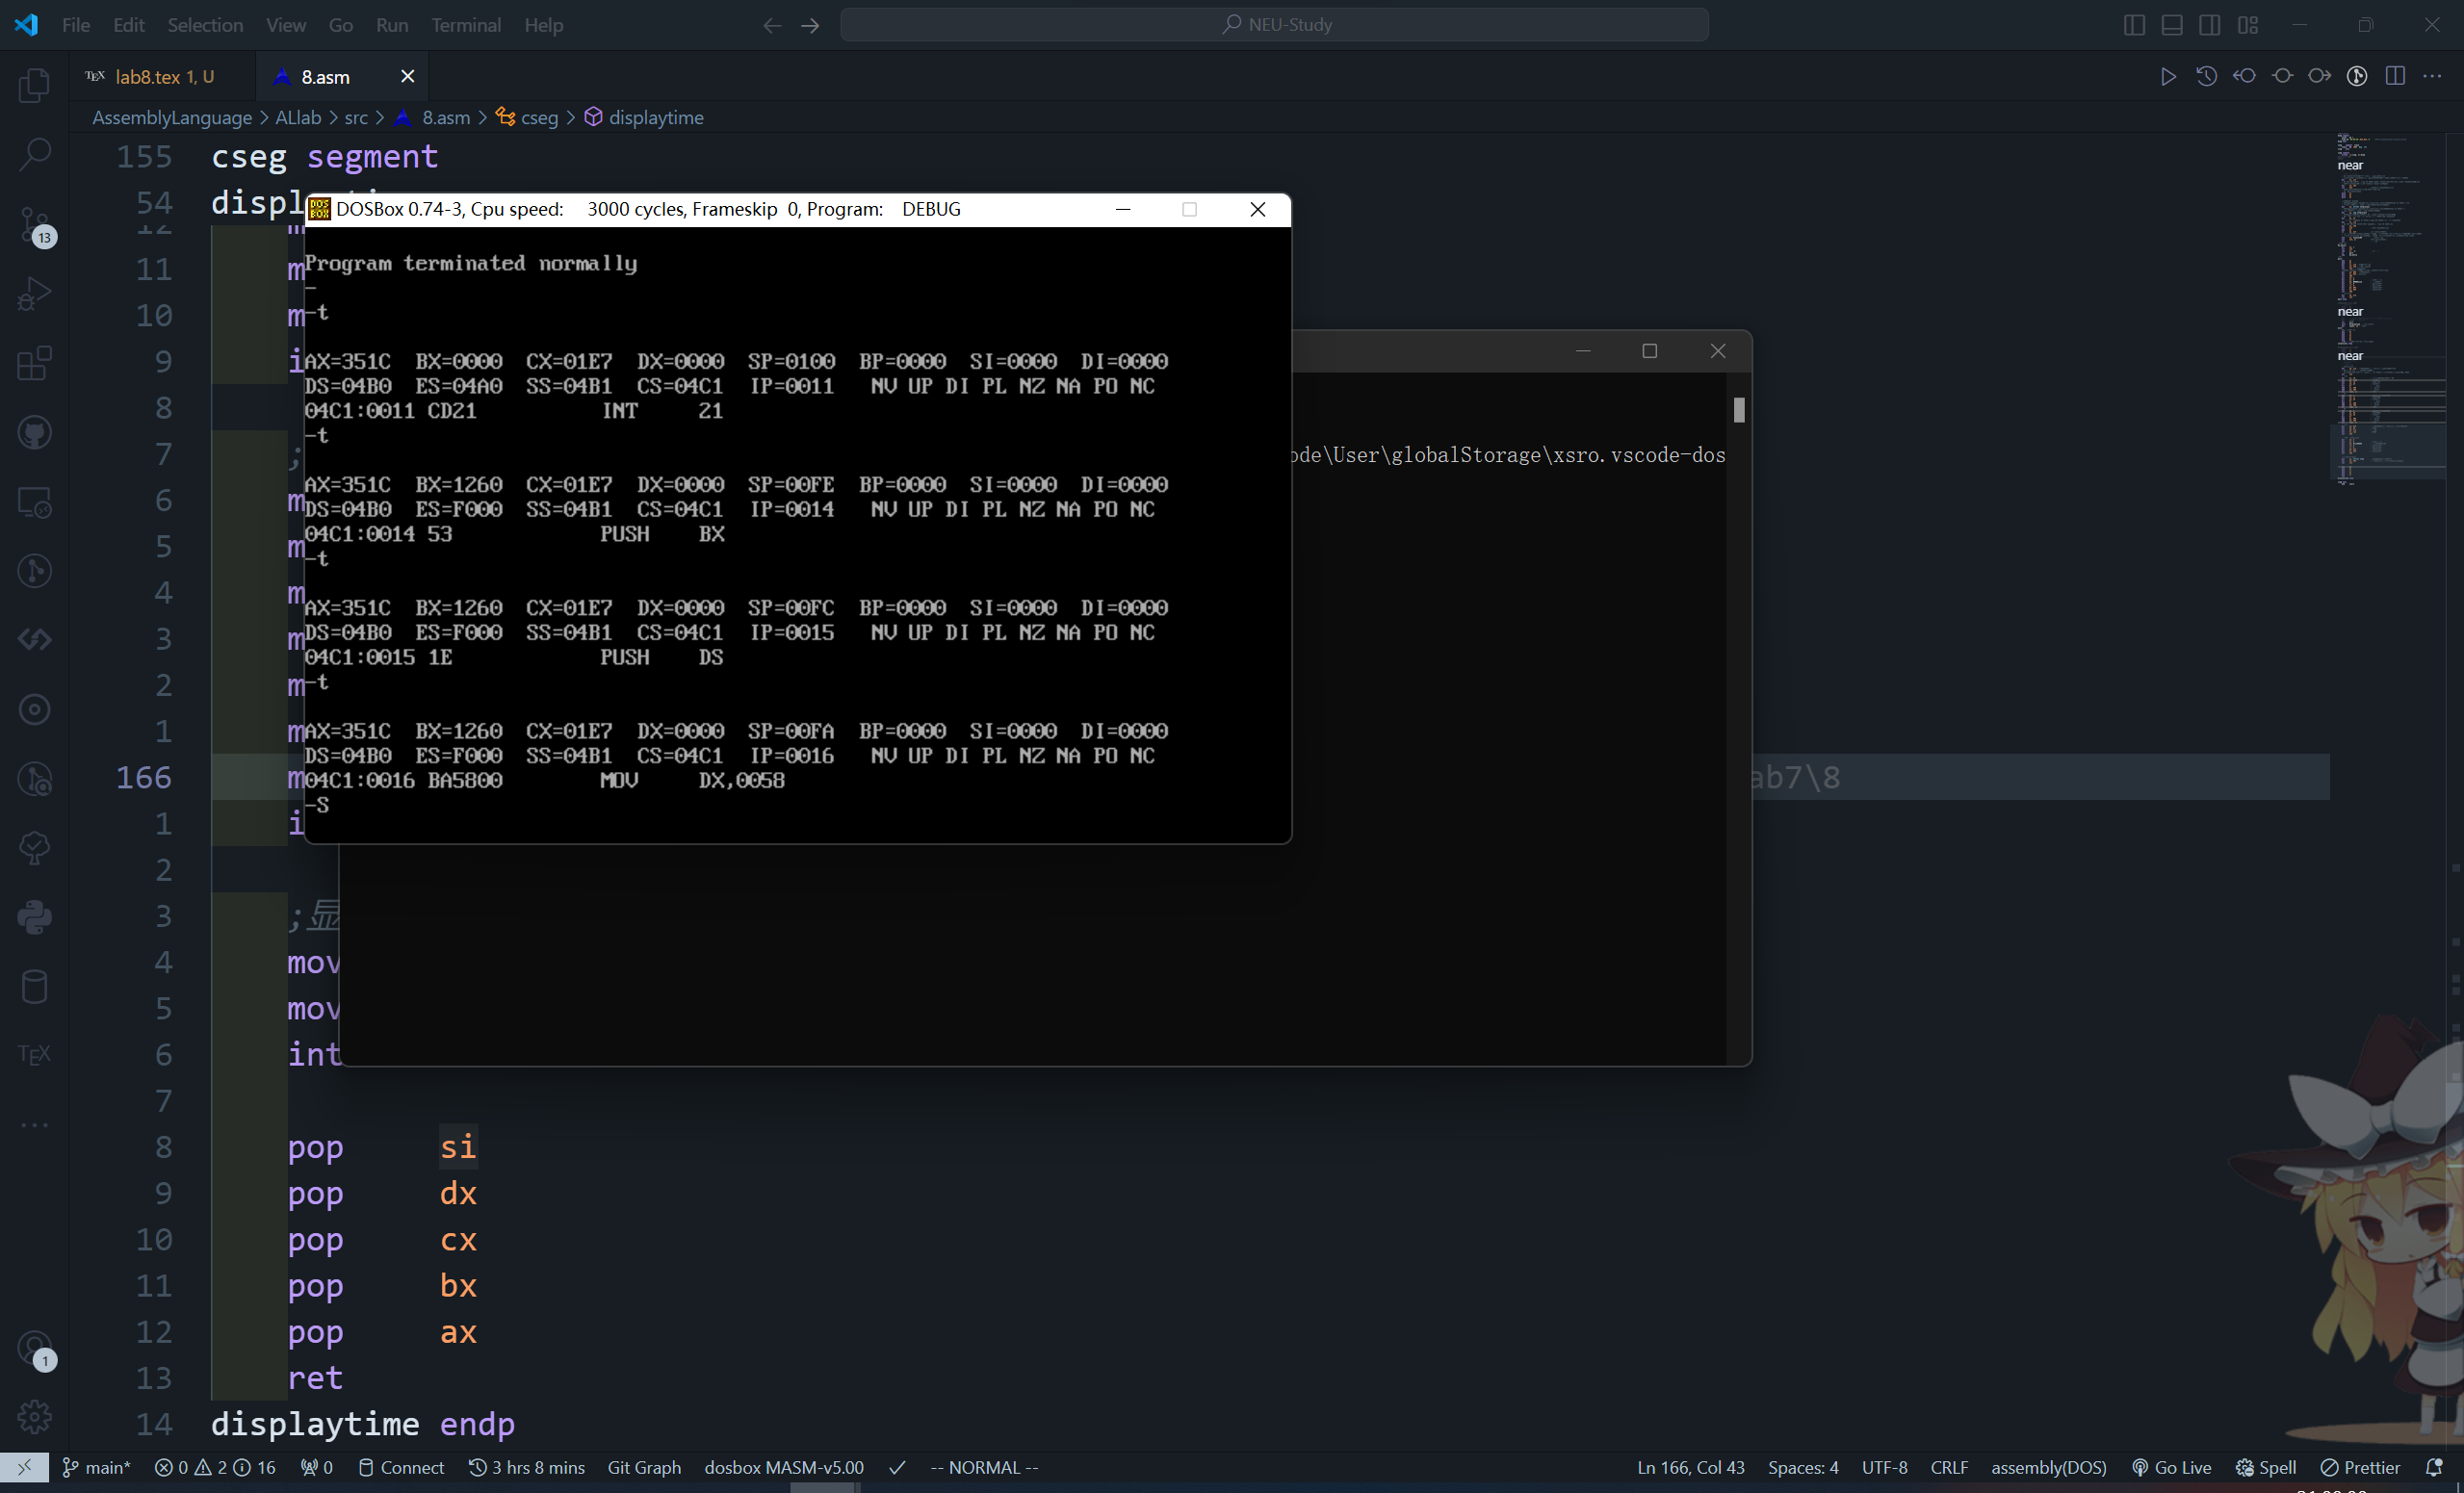
\includegraphics[width=1\textwidth]{image/AL_70.png}\end{center}
    \begin{center}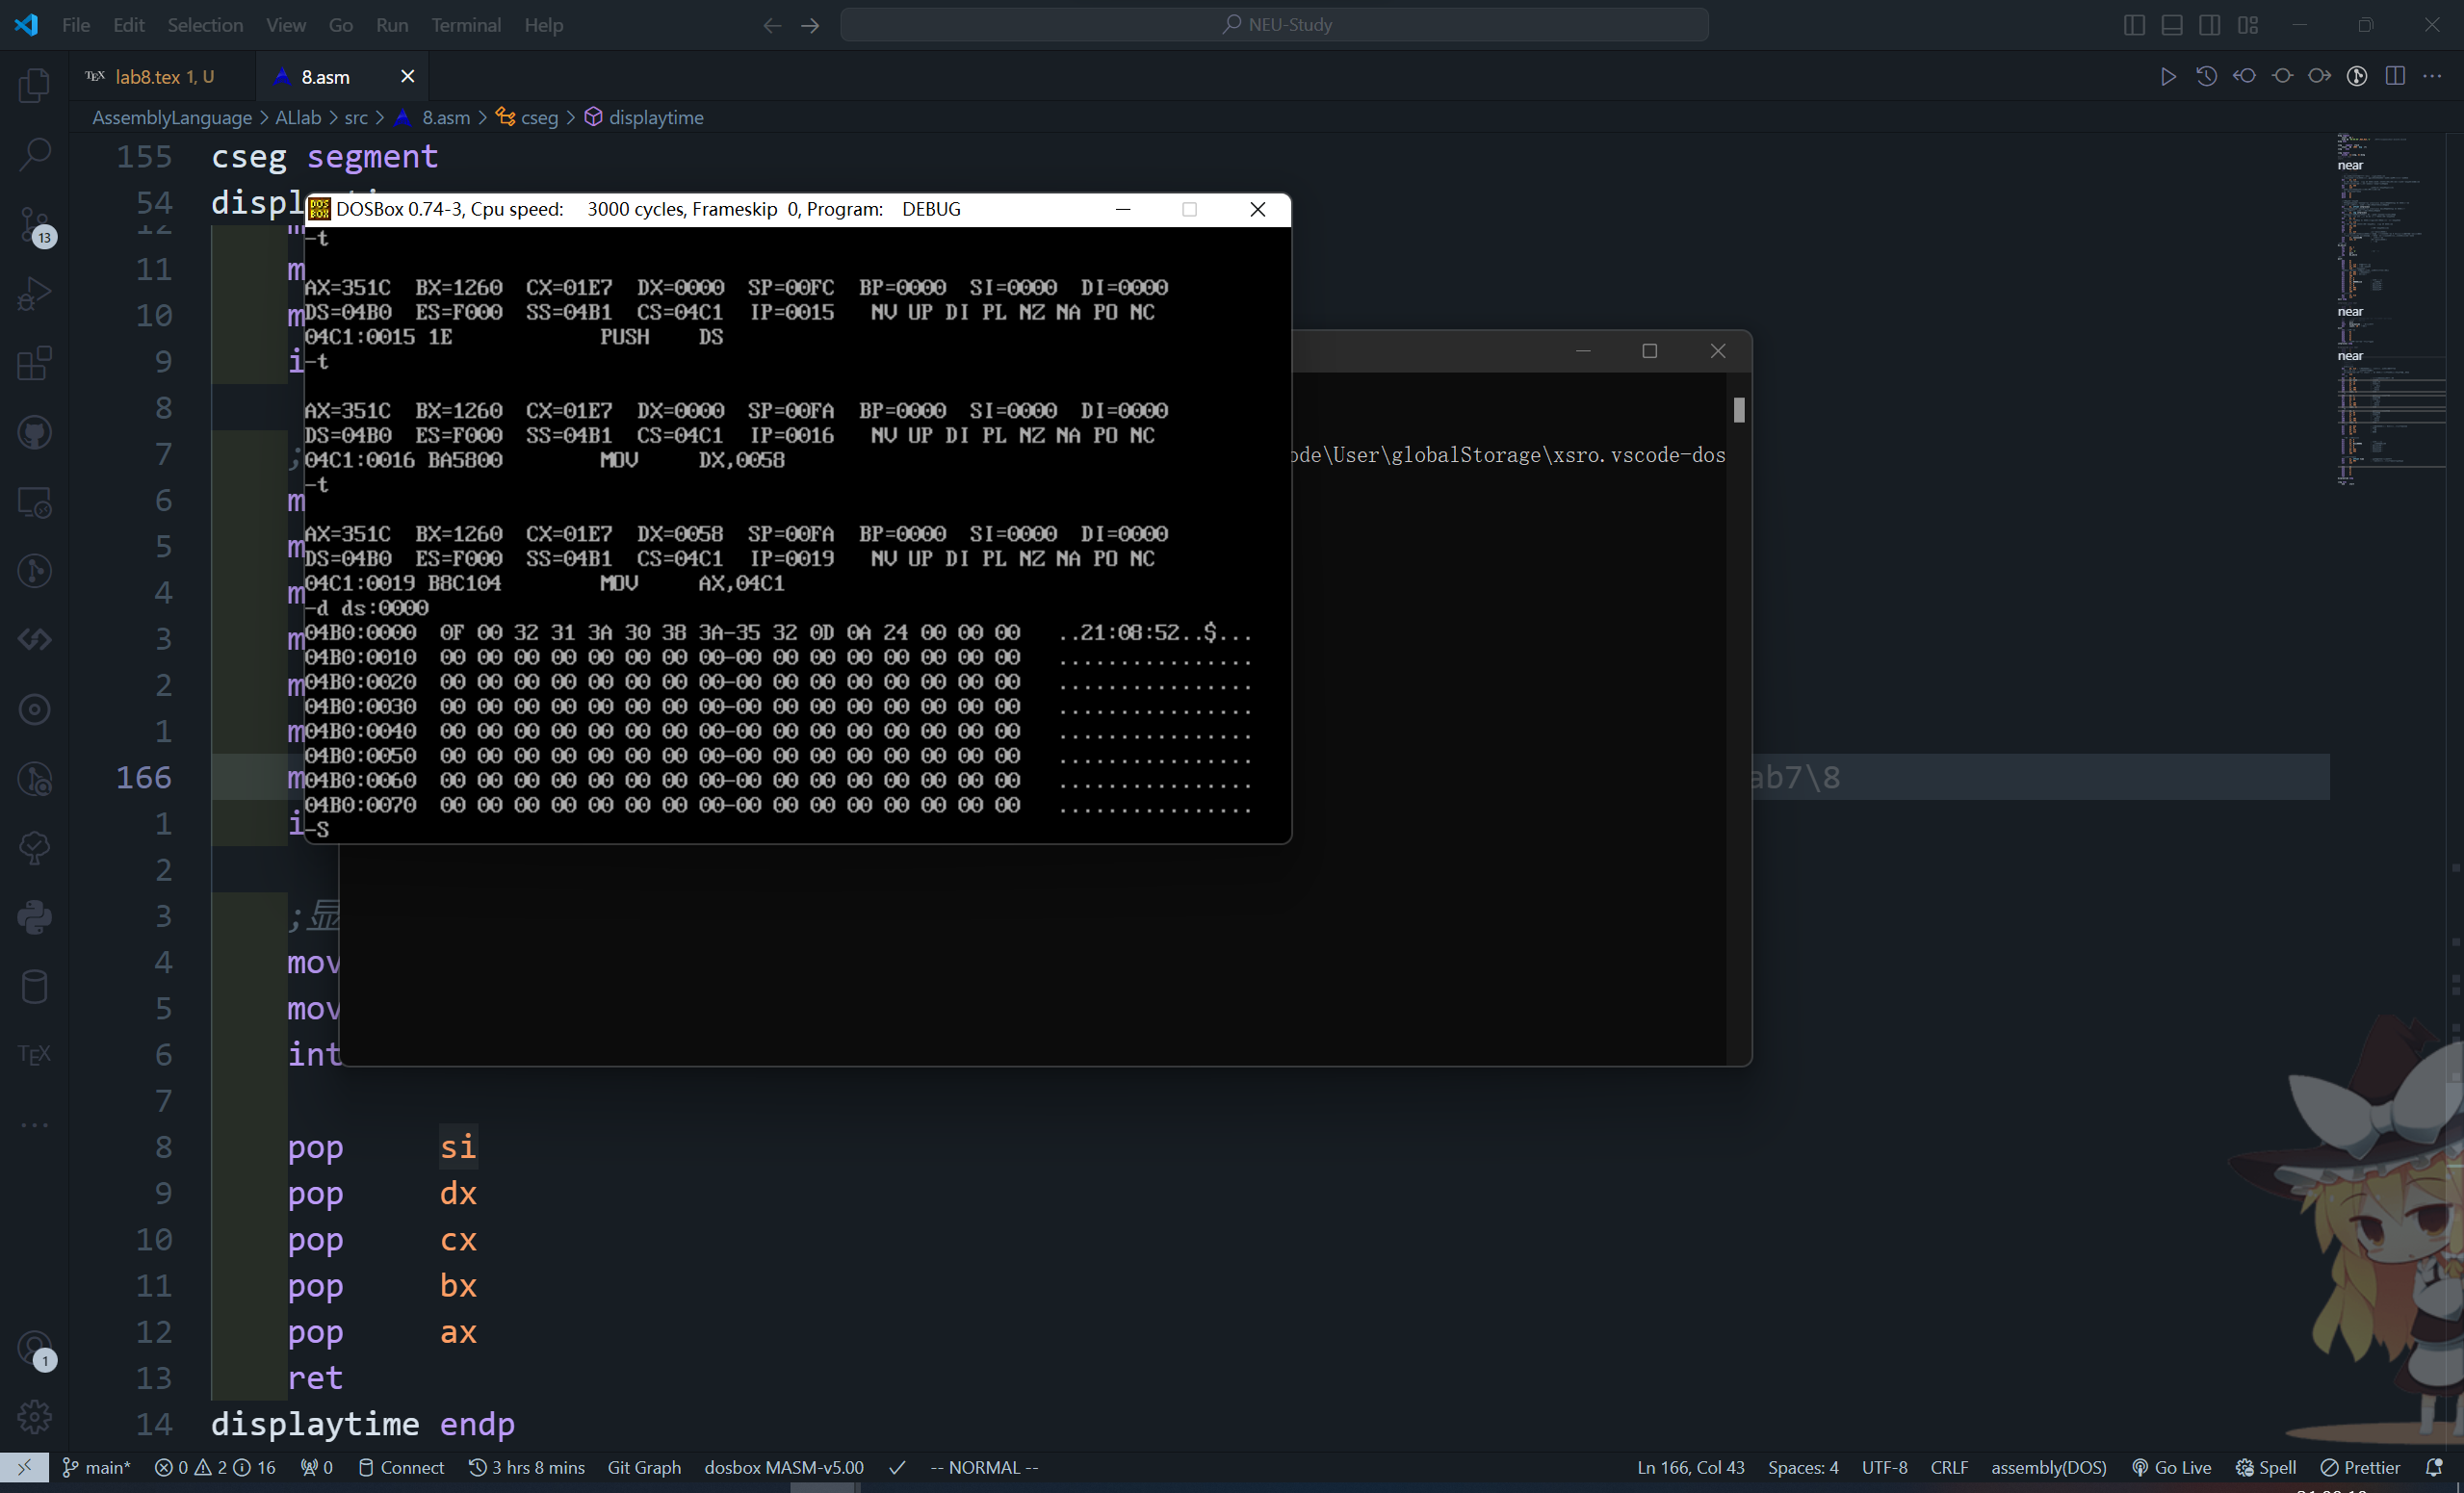
\includegraphics[width=1\textwidth]{image/AL_71.png}\end{center}

    \subsection{显示结果}
    显示结果：
    \begin{center}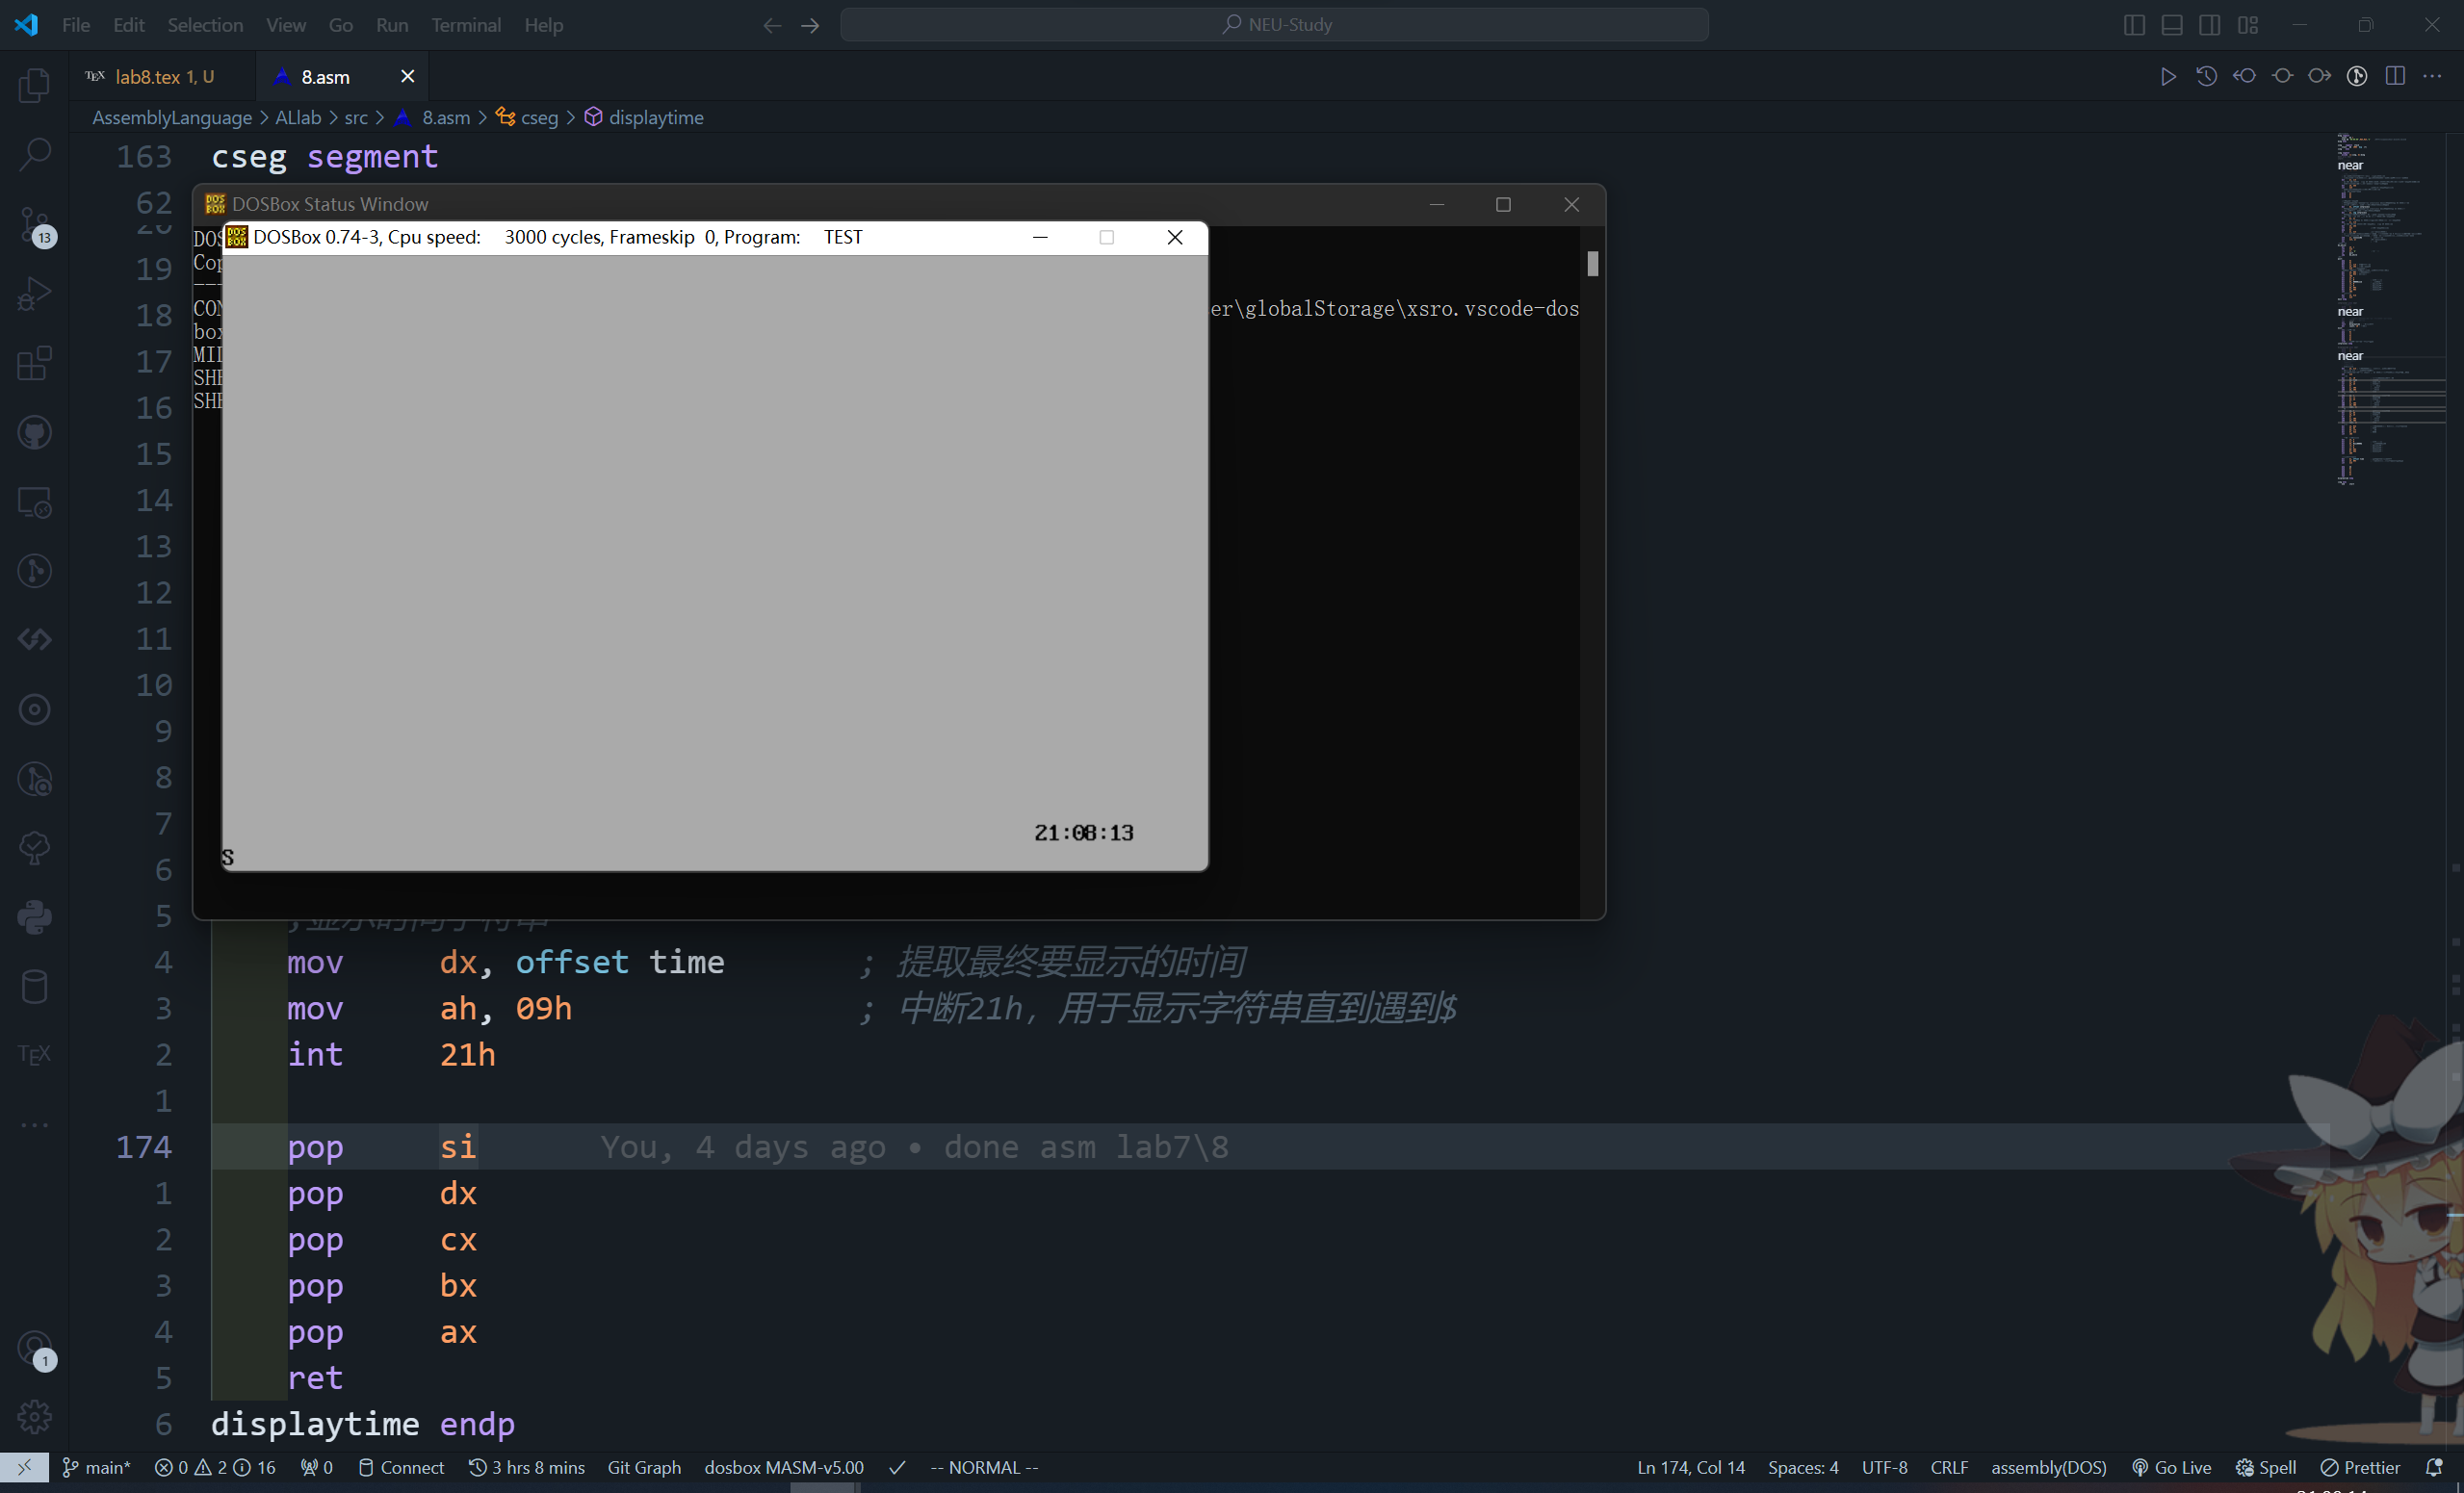
\includegraphics[width=1\textwidth]{image/AL_72.png}\end{center}
    \begin{center}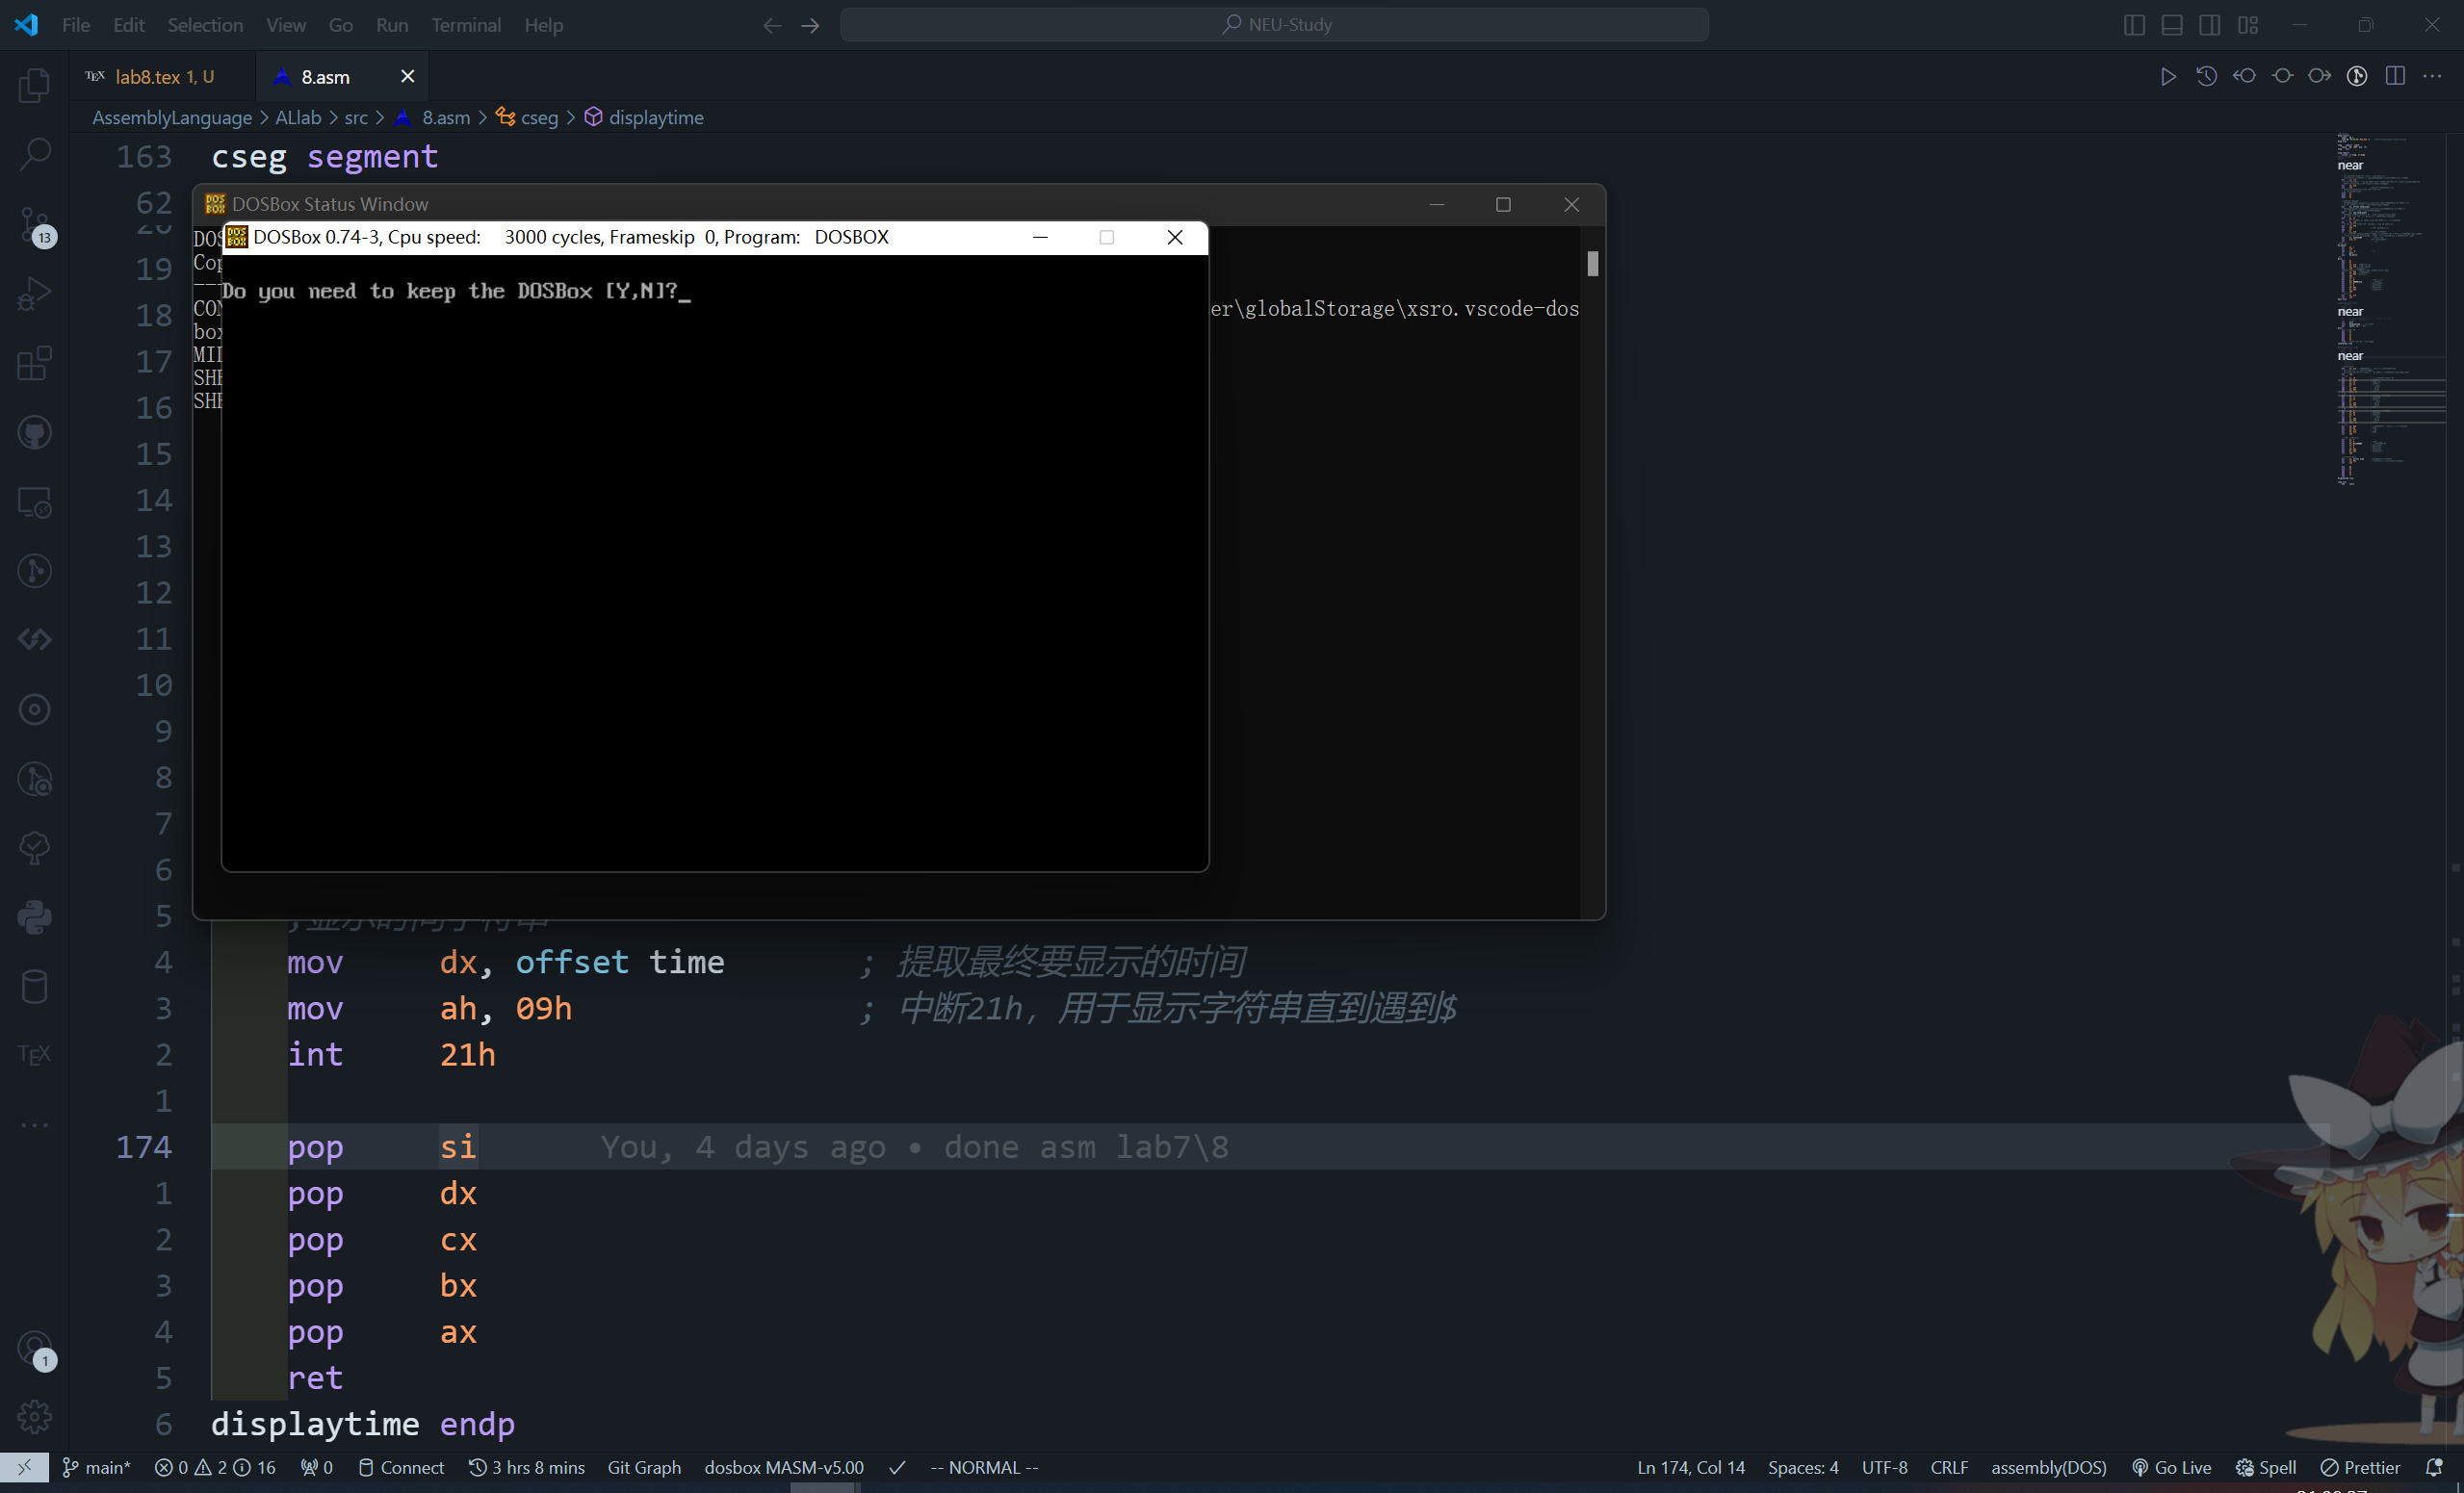
\includegraphics[width=1\textwidth]{image/AL_73.png}\end{center}

    \subsection{流程图}
    \begin{center}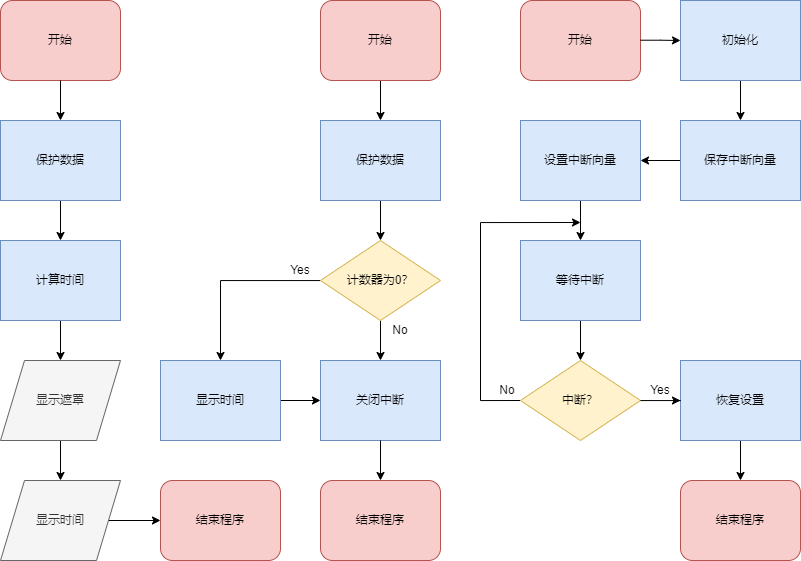
\includegraphics[width=0.8\textwidth]{image/AL_74.png}\end{center}

\section{心得体会}
通过本次实验，我对中断程序设计方法和驻留程序的编写有了更深刻的理解。
这个实验不仅加深了我对理论知识的掌握，也提升了我在实际环境中应用这些知识的能力。

我学习到了如何使用DOS中断编写程序，特别是如何使用和设置中断向量。
通过挂接时钟中断（INT 1Ch），我能够在中断服务程序中更新屏幕上显示的时间，而不影响前台程序的正常运行。
这对于理解操作系统如何管理多个任务和中断非常有帮助。

在实验过程中，我遇到了几个技术挑战，其中最主要的是如何保证时间更新不会影响前台应用的运行。
初期，时间更新时的屏幕刷新导致前台应用出现短暂的闪烁。
为了解决这个问题，我优化了屏幕更新的代码，使用了更有效的屏幕缓冲区处理方法，最终实现了平滑的时间更新显示。

另一个挑战是中断向量的正确管理。
在实验开始时，我没有正确保存和恢复原有的中断向量，这导致在卸载驻留程序后系统行为变得不稳定。
通过仔细阅读相关文档和多次测试，我学会了如何正确处理中断向量，确保程序的稳定性和系统的安全。

此外，这次实验也让我意识到了编写驻留程序时对系统资源的影响。
驻留程序需要非常小心地管理内存和CPU时间，以避免对系统性能造成影响。
通过这次实验，我学会了如何高效地使用系统资源，同时保证程序的响应性和功能性。

这次实验不仅加强了我对中断程序设计的理解，也锻炼了我的问题解决和程序优化能力。
我深刻体会到了理论知识与实际应用之间的联系，这对我的学习和未来的职业生涯都是非常宝贵的经验。

\begin{flushright}\begin{tabular}{rl}
    姓名: & 李俊洁\\
    班级: & 计算机2204 \\
    学号: & 20225443 \\
    课程: & 汇编语言程序设计 \\
    日期: & April 24, 2024 \\
    制作: & \LaTeX \\
    & 感谢您的批阅！
\end{tabular}\end{flushright}
\end{document}